\subsection{Hvad er et Speckle Pattern} 
Speckle patterns betegner et billede eller område prikker af variere størrelse, form og farve. I dette projekt benyttes "speckle pattern"  specifikt til at beskrive et billede med prikker i et tilfældigt mønster, der anvendes ved DIC. Præcisionen af DIC afhænger blandt andet af det anvendte speckle patterns kvalitet, der kan vurderes ved brug af softwareprogrammer. Programmerne benytter forskellige metoder til kvalitets vurdering, der vurderer parametre som størrelse, form og fordeling af prikkerne. Et godt speckle pattern er karakteriseret ved høj kontrast mellem prikker og baggrund, tilfældigt mønster der er jævnt fordelt og udgør mellem 50\% og 70 \% af billedet. Prikkerne skal have en konsistent radius, samt have en størrelse på mellem 3x3 og 5x5 pixels. Derudover skal prikkerne være indenfor kameraets field of view (FOV). (\cite{Dong2017ACorrelation}; \cite{Su2022Glare:Pattern}; \cite{Gagnon2024ThePatterns}).  


%------
\paragraph{Høj kontrast} DIC benytter gray level til vurdering af prikkernes placering på overfladen. Gray level er en grå-skala værdi fra 0\% til 100\%, der beskriver lysintensiteten i et enkelt pixel. Et Gray level på 100\% ses som hvid, hvor 0\% er helt sort, fordi der gray level værdien angiver mængden af lys. Det er derfor nødvendigt med høj kontrast mellem prikker og baggrund, så kameraet kan opfange forskellen mellem prikker og baggrund. Oftest gøres brug af sorte prikker på hvid baggrund, eller hvide prikker på sort baggrund, idet disse har største forskel mellem prikkerne og baggrundens gray lavel. (\cite{Reu2015AllContrast})


%-----
\paragraph{Størrelse på prikkerne} Prikkernes størrelse har betydning for, hvordan prikkerne opfanges af kameraet samt softwaren der benyttes til DIC. For et optimalt resultat skal prikkerne være større end 3 pixels, hvilket afhænger af kameraets opløsning og FOV. Den minimale diameter på prikkerne {$d_{min}$}, er derfor afhængig af FOV og antallet af pixels ($n_{pixels}$), som det fremgår af formel \ref{equ:prikstørrelse-d_min}. FOV definere enten bredden eller højden på området indenfor kameraets synsfelt, der er påført speckle pattern, og måles i millimeter. Formlen bruges til at give et estimat af den minimale diameter prikkerne må have, for at give et optimalt resultat ved DIC. $d_{min}$ beregnes seperat for henholdsvis bredden og højden af FOV. Hvis $d_{min}(bredden) \neq d_{min}(hoejden)$, benyttes den største diameter (\cite{Reu2014AllAliasing}).
 \begin{equation} \label{equ:prikstørrelse-d_min}
     d_{min} = \frac{FOV}{n_{pixels}} \cdot 3 \ pixels
 \end{equation}
Prikker mindre end 3 pixels er vanskelige at bestemme centrum af, idet en prik på 1 pixels der ligger mellem 2 pixels vil give en slørret afbildning i gray level, hvorved kontrasten mellem prik og baggrund mindskes, hvilket medfører en stigning i systematiske fejl. Yderligere øges præcisionen ved brug af prikker over 3 pixels, fordi det bliver tydeligere på gray level, hvor prikken er lokaliseret, da de vil fremgå af flere pixels, solom prikken er placeret mellem to pixels. (\cite{Reu2014AllAliasing}; \cite{Cui2024EffectError})

Prikkerne kan ikke være uendeligt store, og er begrænset af FOV, kameraets opløsning og det procentvise forhold prikkerne må dække af hele overfladen samt størrelsen på overfladen der undersøges. Tracking af mindre deformationer vanskeliggøres, ved brug af store prikker, samtidig med, at softwaren generelt har sværere ved at finde den enkelte prik før og efter  deformation. Dette skyldes, at DIC gør brug af de øvrige pixels i FOV, for at finde frem til en bestemt prik, hvilket er vanskelige ved store prikker, der medfører et mindre antal af prikker i FOV. Prikkerne optimale størrelse er under 5x5 til 7x7 pixels. (\cite{Haddadi2008UseTechnique}; \cite{Crammond2013SpeckleCorrelation}; \cite{Dong2017ACorrelation}; \cite{Gagnon2024ThePatterns}).
 \begin{equation} \label{equ:prikstørrelse-d_max}
     d_{maks} = \frac{FOV}{n_{pixels}} \cdot 7 \ pixels
 \end{equation}
Ved forventning om store deformationer, hvor mindre deformationer er uvæsentlige at undersøge, kan større prikker bruges, uden det har betydning for det der ønskes undersøgt. Overfladens størrelse  medvirker til den maksimale størrelse $d_{maks}$ prikkerne kan have, idet store overflader, kan benytte prikker af en større størrelse end små samples til materialetest, fordi FOV er større. Prikkerne i det samme speckle pattern kan variere mellem 3 pixels og 7 pixels, men for optimal måling skal størrelsesforskellen på prikkerne i det samme speckle pattern holdes minimal(\cite{Crammond2013SpeckleCorrelation}; \cite{Gagnon2024ThePatterns}).  

%-----
\paragraph{Tilfældigt og isotropt} Identifikationen af en enkelt priks bevægelse under deformation af emnet, er kun mulig, hvis prikkerne er arrangeret i et mønster der ikke gentages.  (\cite{Zaya2023ApplicationReview}).

%----
\paragraph{Fordeling af prikkerne} Et godt speckle pattern har en 50\% til 70\% fordeling af henholdsvis prikker og baggrund. Prikkerne skal være jævnt fordelt med minimum 3 pixels mellem alle prikkerne. HVis prikkerne er for tætte på hinanden, så kan softwaren have vanskeligt ved, at indentificere om det er én stor prik eller flere små prikker, hvilket øger usikkerheden ved måling. (\cite{Reu2015AllDensity}; \cite{Caliskan2024InvestigationDIC})

\begin{figure}[H]
  \centering
    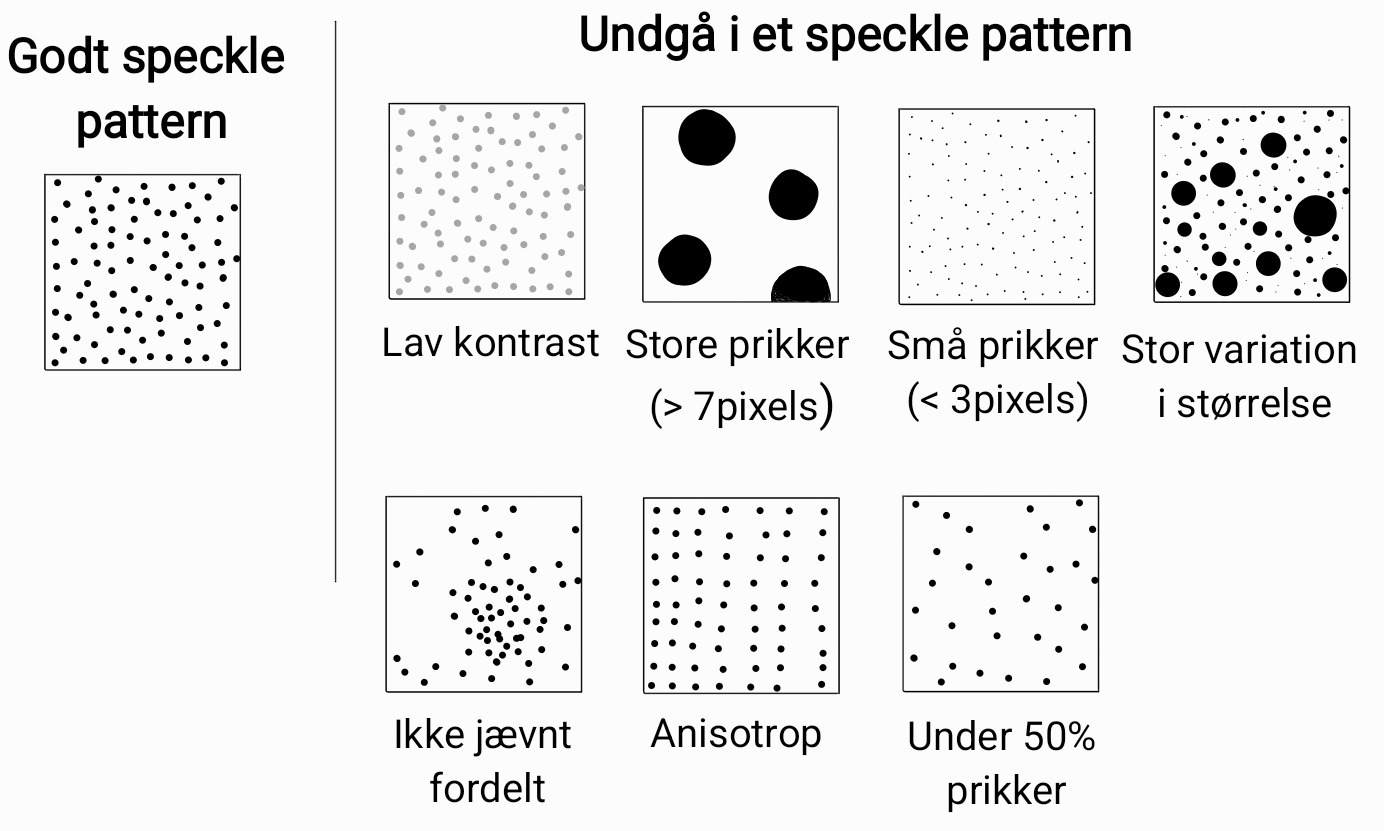
\includegraphics[width=0.8\textwidth]{Sections/2 Problemanalyse/Media/Speckle pattern.jpg}
    \caption{Illustration af fejlkilder ved produktion af speckle pattern til DIC.}
    \label{fig:godt speckle pattern}
\end{figure}

Figur \ref{fig:godt speckle pattern} illustrere fejlkilder i speckle patterns der mindsker præcisionen af DIC. Kriterierne for et godt speckle pattern er gældende for både 2D og 3D.


%-----
\paragraph{Forblive på overfladen} Det er nødvendigt, at prikkerne forbliver på og deformerer med overfladen af genstanden der undersøges. Resultaterne af DIC er ikke retvisende, hvis prikkerne flytter sig uafhængigt af det undersøgte materiale, derfor er det nødvendigt, at prikkerne flytter sig med materialet. Derudover skal prikkerne ikke have tydelig ændring i gray level eller geometri
(\cite{Dong2017ACorrelation} ; \cite{Zaya2023ApplicationReview}).





\begin{comment}
Antallet af prikker der forekommer i et computer genereret speckle beskrives ud fra formel \ref{equ: antal prikker}. $\rho$ er densitet. r er prikkernes radius. w er bredden af billedet, der også kan erstattes af h, som er højden af billedet. (\cite{Cui2024EffectError}) 
 
 \begin{equation} \label{equ: antal prikker}
     n=\frac{\rho w}{2r}
 \end{equation}

 
\begin{figure}[H]
  \centering
    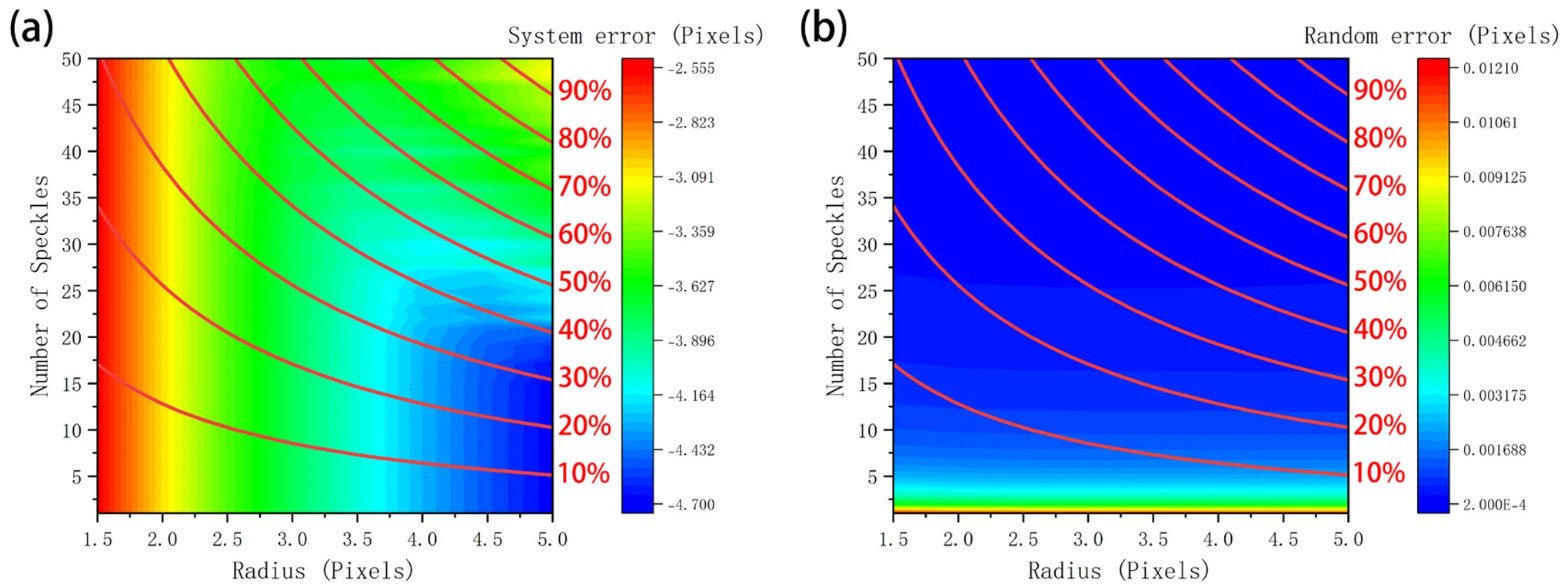
\includegraphics[width=0.8\textwidth]{Sections/1 Problemanalyse/Media/error i speckles.png}
    \caption{Antal prikker i et manuelt genereret speckel pattern på 512 pixels x 512 pixels. Billedet fra (\cite{Cui2024EffectError}).}
    \label{fig: error ved speckel pattern}
\end{figure}
\end{comment}




 


